\documentclass[10pt,a4paper]{article}
\usepackage[utf8]{inputenc}
\usepackage[T1]{fontenc}
\usepackage{lmodern}
\usepackage[margin=1.5cm, top=1.4cm, bottom=1.4cm]{geometry}
\usepackage{hyperref}
\usepackage{enumitem}
\usepackage{titlesec}
\usepackage{xcolor}
\usepackage{graphicx}

\definecolor{accent}{HTML}{00686E}
\hypersetup{colorlinks=true, urlcolor=accent, linkcolor=accent}
\pagenumbering{arabic}
\setlength{\parindent}{0pt}

\titleformat{\section}{\large\bfseries\color{accent}}{}{0em}{}[\vspace{-0.6em}\rule{\textwidth}{0.8pt}]
\titlespacing{\section}{0pt}{7pt}{4pt}

\newcommand{\role}[4]{%
  \textbf{#1} \hfill \textbf{#2}\\[1pt]%
  \textit{#3} \hfill \textit{#4}\\[2pt]%
}
\setlist[itemize]{leftmargin=1.2em, itemsep=1.5pt, topsep=2pt, parsep=0pt}

\begin{document}

% ================= HEADER =================
\begin{minipage}[c]{0.80\textwidth}
  {\Huge\bfseries Prabhavit Gupta}\\[3pt]
  {\color{accent}\large Senior Full-Stack \& AI Engineer: Multi-LLM APIs \& Evaluation Pipelines}\\[6pt]
  {\footnotesize +39 351 610 7807 ~$\vert$~
  \href{mailto:prabhavitg@gmail.com}{prabhavitg@gmail.com} ~$\vert$~
  \href{https://www.linkedin.com/in/prabhavit/}{linkedin.com/in/prabhavit} ~$\vert$~
  \href{https://github.com/prab-gupta}{github.com/prab-gupta} ~$\vert$~
  Venice, Italy (CET Time Zone / EU Permanent Resident)}
\end{minipage}\hfill
\begin{minipage}[c]{0.18\textwidth}
  \raggedleft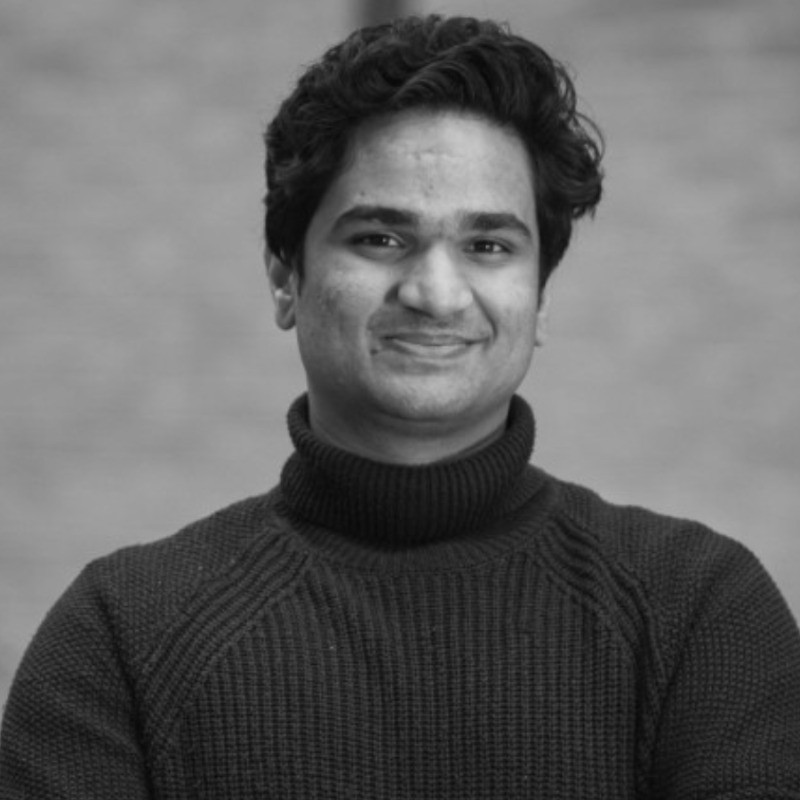
\includegraphics[width=2.0cm]{photo.jpg}
\end{minipage}
\vspace{-2pt}

% ================= SUMMARY =================
\section{Summary}
Full-Stack and AI Engineer with 3 years of hands-on production experience architecting large-scale multi-LLM API interaction systems, automated model evaluation pipelines, and high-integrity data provenance layers. Extensive practical experience executing comparative evaluations across frontier models (Claude, ChatGPT, Gemini), building structured evidence capture pipelines, and optimizing distributed ingestion services. Proficient across TypeScript, Python, PostgreSQL, and modern vector retrieval architectures. Based in Venice, Italy (CET time zone) with an EU Long-Term Residence Permit (permanent unrestricted EU work authorization, no sponsorship required); available immediately for full-time remote roles.

% ================= TECHNICAL EXPERTISE =================
\section{Technical Expertise}
\begin{itemize}
  \item \textbf{Multi-LLM APIs \& Evaluation:} Large-scale LLM querying (Claude, OpenAI, Gemini), automated evaluation harnesses, prompt comparison, semantic scoring, hallucination detection, rate-limit management.
  \item \textbf{Data Provenance \& Extraction:} Structured evidence capture, snapshot validation, immutable audit logs, web scraping and DOM extraction with Playwright, schema validation with Pydantic and Zod.
  \item \textbf{Full-Stack \& Backend Engineering:} TypeScript, Node.js, Python (FastAPI, asyncio, pandas, NumPy), RESTful API design, microservices, asynchronous task queues (Redis).
  \item \textbf{Data Stores \& Infrastructure:} PostgreSQL (relational modeling, JSONB indexing, high-concurrency read/write), vector databases, Docker containerization, GitOps, CI/CD pipeline automation.
  \item \textbf{Reliability \& Testing:} Automated contract and regression testing with Playwright, distributed tracing, structured logging, latency profiling, and cost engineering.
  \item \textbf{Languages \& Authorization:} English (C1 Professional, fluent), Hindi (Native), Italian (Beginner). EU Long-Term Residence Permit (unrestricted EU work authorization across all EU member states, no sponsorship required).
\end{itemize}

% ================= EXPERIENCE =================
\section{Experience}

\role{\href{https://flowspace.co}{FlowSpace.co}}{Mar 2024 - Aug 2026}{Lead Developer \& AI Systems Architect}{London, UK (remote)}
\begin{itemize}
  \item Designed and operated production multi-LLM querying pipelines and data extraction systems for an enterprise platform serving 4,500+ active users.
  \item Built automated evaluation and benchmarking harnesses evaluating model responses across multiple LLM providers against gold-standard evaluation datasets.
  \item Implemented structured evidence capture and data provenance pipelines, recording inputs, outputs, timestamps, and model parameters into PostgreSQL.
  \item Engineered resilient asynchronous processing queues with Redis, handling high-throughput parallel API requests while adhering to strict provider rate limits.
  \item Developed automated validation test suites with Playwright to verify continuous data extraction accuracy and prevent regressions.
  \item Architected high-performance TypeScript and Python backend services, optimizing data serialization and decreasing query response latency.
\end{itemize}

\role{Urlink}{Apr 2025 - Jul 2025}{Project Manager \& Solutions Developer (Freelance)}{Barcelona, Spain (remote)}
\begin{itemize}
  \item Delivered custom full-stack applications and automated data processing services for European client platforms using TypeScript, Node.js, and PostgreSQL.
  \item Built ETL ingestion services connecting external APIs, ensuring verified data transformation and provenance.
  \item Created interactive prototypes and automated validation checks to verify functional specifications prior to production delivery.
\end{itemize}

\role{Independent Technical Consultant}{Aug 2023 - Feb 2024}{AI Automation \& Integration Developer}{Venice, Italy}
\begin{itemize}
  \item Developed custom Python utilities and webhook integrations querying multiple LLM APIs for automated classification and sentiment analysis.
  \item Built robust data validation routines ensuring incoming unstructured web content conformed to rigorous relational database schemas.
  \item Authored technical architecture specifications, API documentation, and deployment guides for client engineering teams.
\end{itemize}

% ================= EDUCATION =================
\section{Education}
\role{Ca' Foscari University of Venice}{2020 - 2024}{BA in Philosophy, International Studies and Economics}{Venice, Italy}
\begin{itemize}
  \item Rigorous training in formal logic, analytical problem solving, systems analysis, and macroeconomic decision models.
\end{itemize}

\end{document}
